\chapter{Обзор алгоритмов управления скоростью}
\label{cha:chap2}

\section{ПИ (ПИД) регулятор}
\label{sec:pid}

В качестве простейшего регулятора скорости может быть использован одноконтурный ПИ или ПИД регулятор по скорости. Схема реализации приведена на Рисунке \ref{pic:pid1}.

\begin{figure}[!h]
\centering
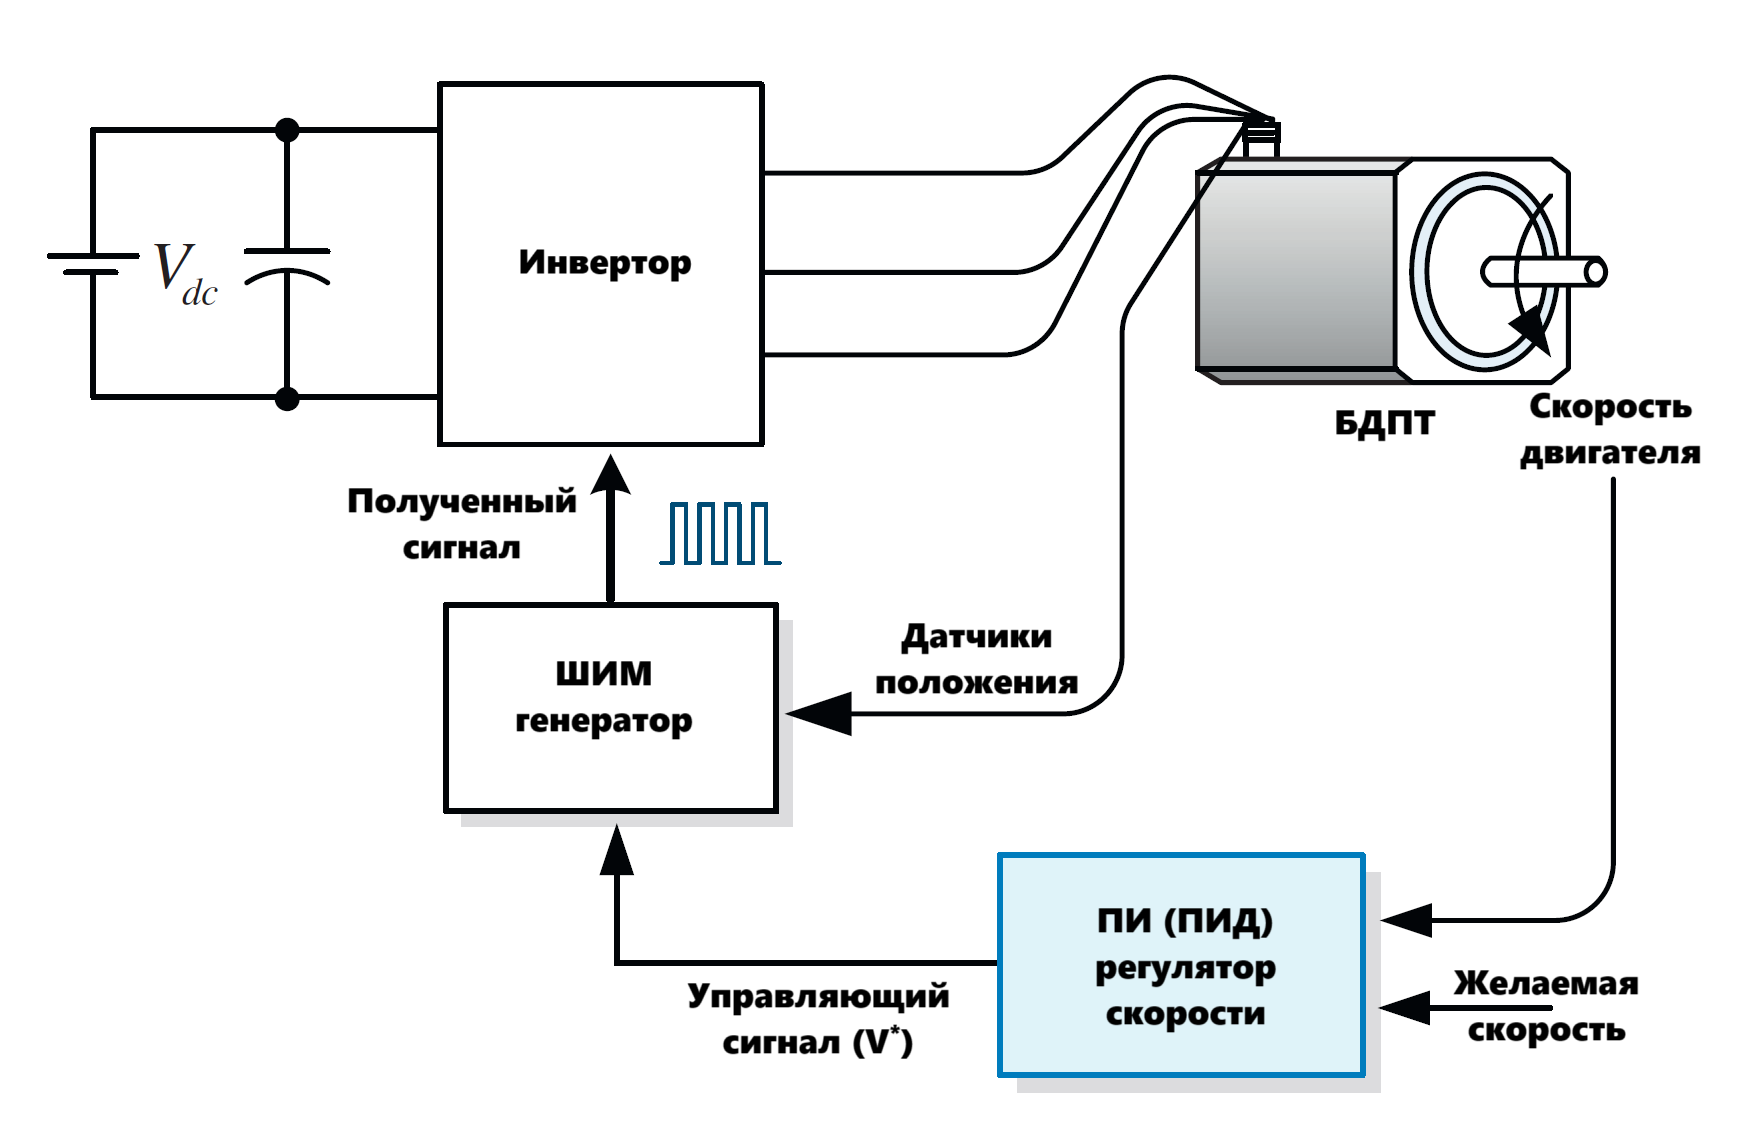
\includegraphics[width=0.7\textwidth]{inc/img/pid1.png}
\caption{Одноконтурная система регулирования скорости \cite{book.kim_motors}}
\label{pic:pid1}
\end{figure}

Данная реализация требует наличия только показаний с датчиков положения двигателя. Однако, использование системы без регулирования тока или момента может вызвать скачки по току, что может вызвать выход из строя системы, не рассчитанной на такой ток. Для исправления этого можно добавить второй контур регулирования по току. Схема реализации приведена на Рисунке \ref{pic:pid2}

\begin{figure}[!h]
\centering
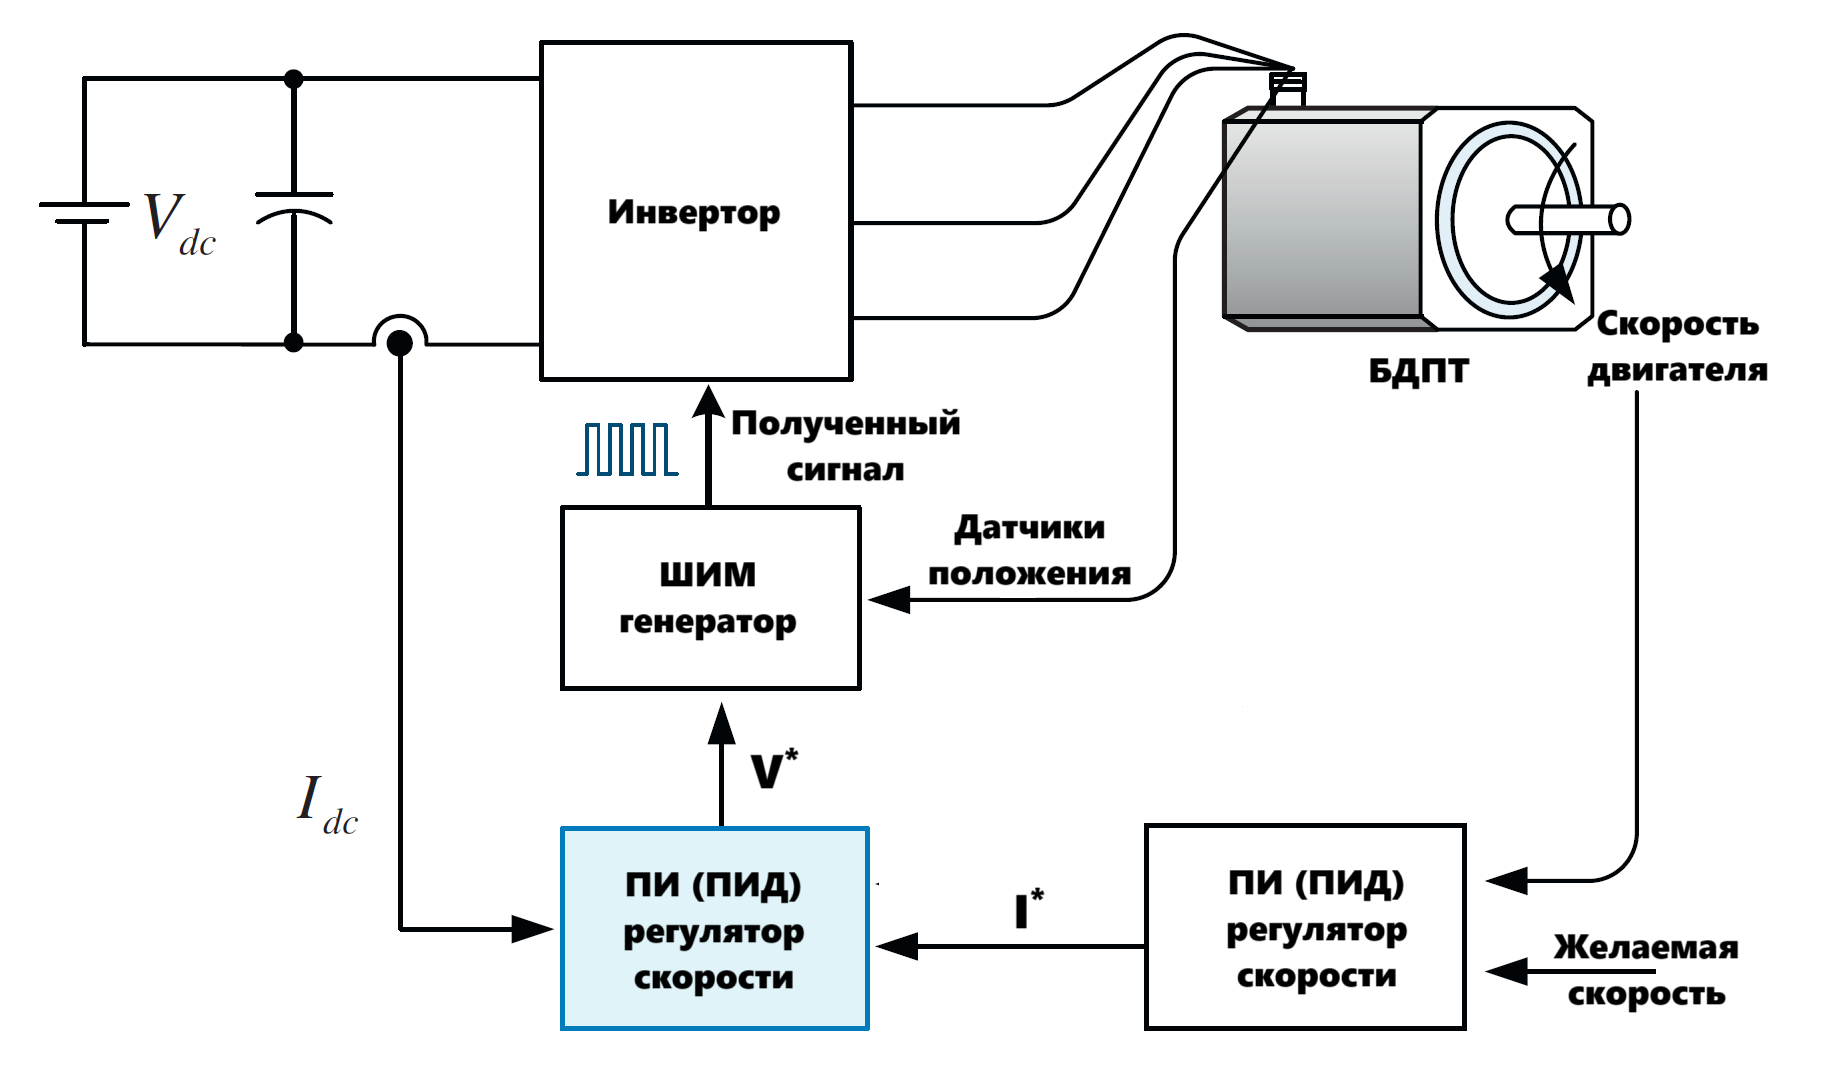
\includegraphics[width=0.7\textwidth]{inc/img/pid2.png}
\caption{Двухконтурная система регулирования скорости \cite{book.kim_motors}}
\label{pic:pid2}
\end{figure}

Для этого подхода необходимо в систему помимо датчиков положения ротора добавить датчик тока.

Использование второго контура позволяет ограничить пульсации тока (момента) во время коммутации (смены питаемых обмоток). Но на практике у нас всё равно появляются пульсации момента, вызванные несколькими причинами: особенностями структуры двигателя (несинусоидальный ток и противо-ЭДС из-за питания от постоянного тока и 6-шаговой алгоритмом управления), неэффективной коммутацией во время смены фаз. Особенно пульсации момента наблюдаются во время постоянно меняющейся нагрузки. На Рисунке \ref{pic:commut} приведены графики изменения момента во время коммутации на различных скоростях.

\begin{figure}[!h]
\centering
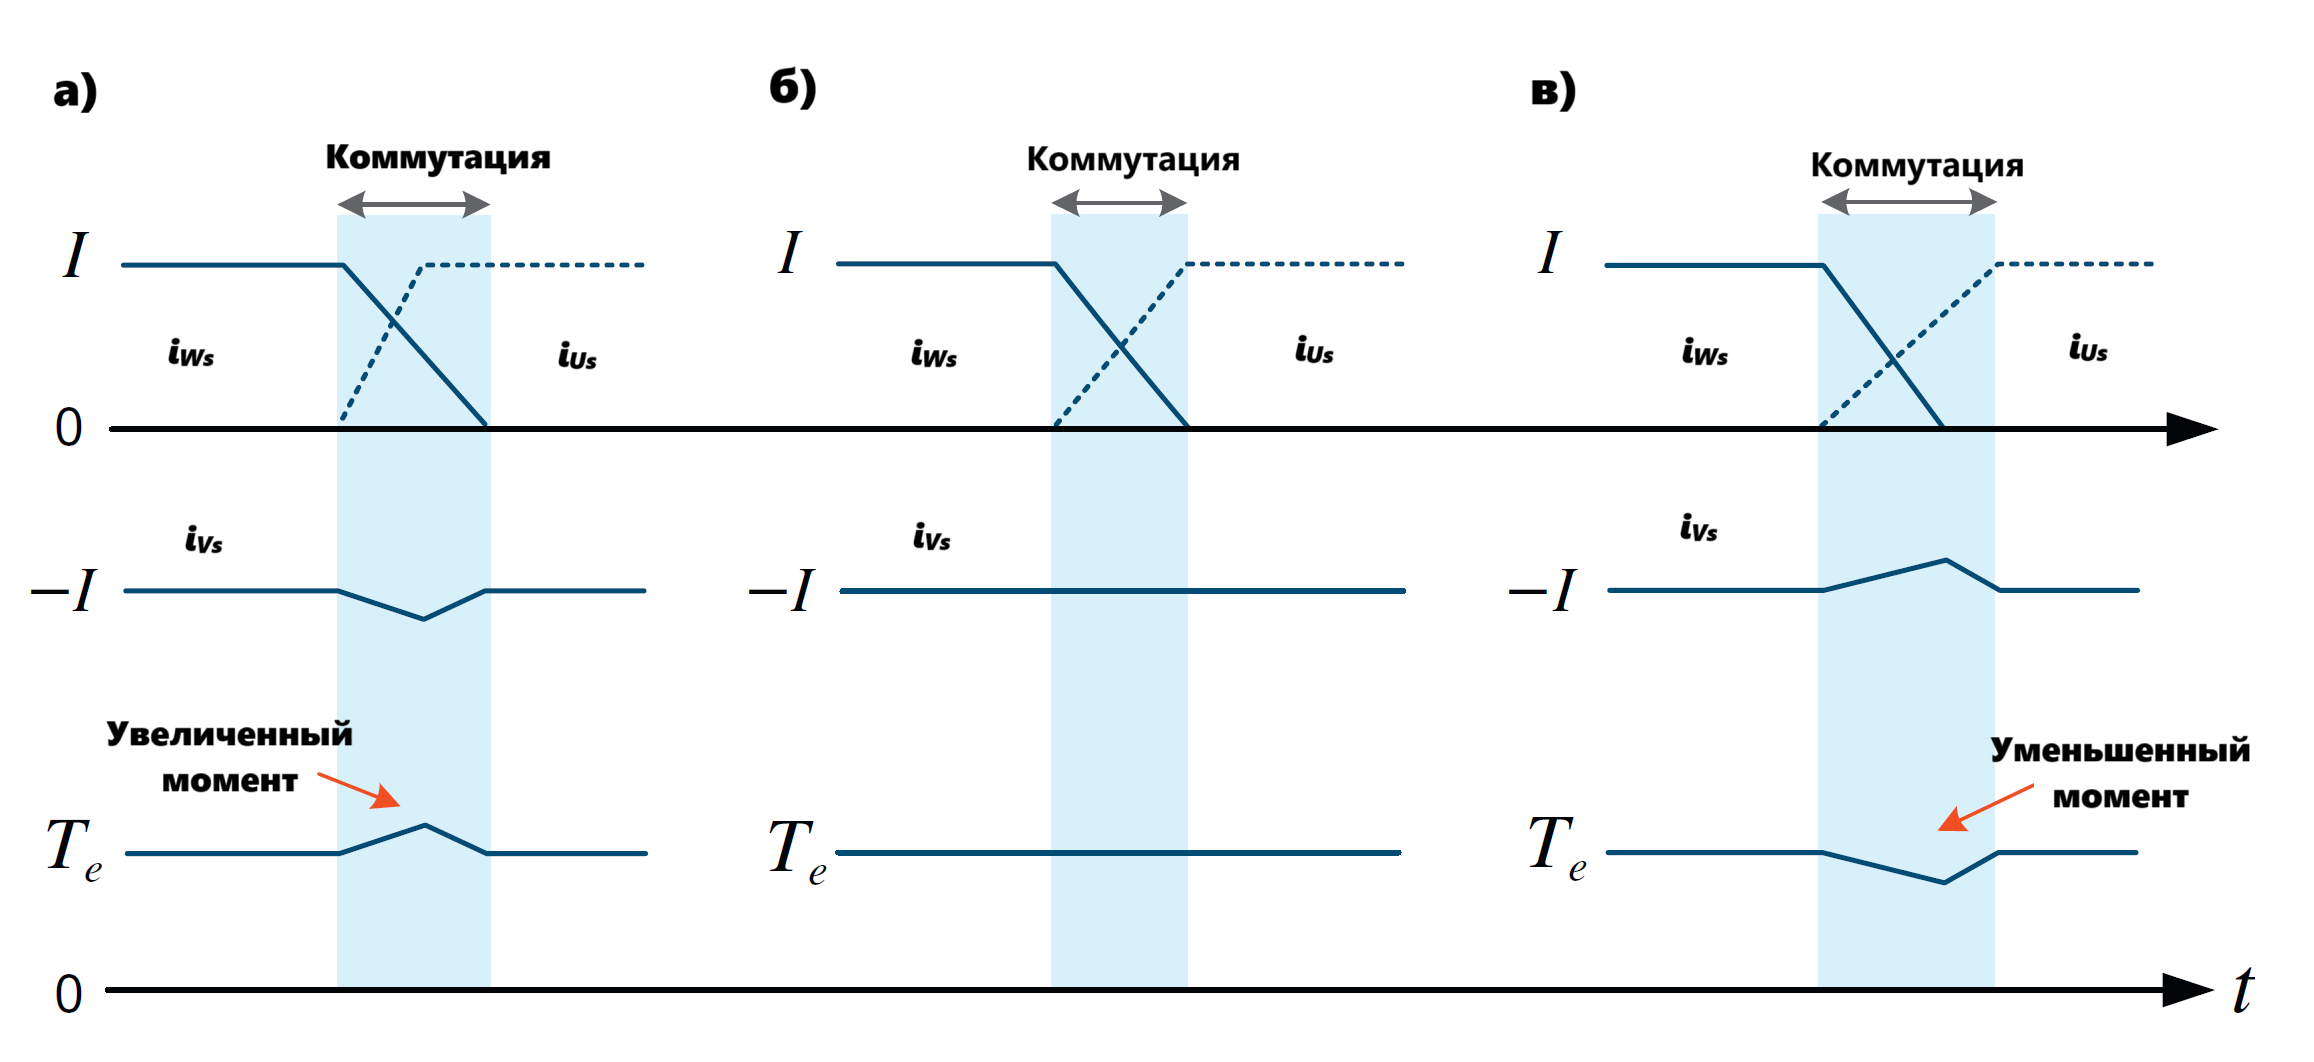
\includegraphics[width=\textwidth]{inc/img/torque_ripple.png}
\caption{Пульсации момента БДПТ на различных скоростях (а --- малые скорости ($V_{dc}>4E$), б --- средние скорости ($V_{dc}=4E$), а --- высокие скорости ($V_{dc}<4E$) ($E$ --- амплитуда противо-ЭДС)) \cite{book.kim_motors}}
\label{pic:commut}
\end{figure}

Для решения этой проблемы используются алгоритмы, рассмотренные далее.

\section{Векторное управление (FOC)}
\label{sec:foc}

Одной из самых ранних техник для уменьшения пульсаций момента является векторное управление или field orientation control (FOC). Данный алгоритм используется для независимого управления тремя параметрами двигателя (скорость, потокосцепление и момент) и позволяет получить форму тока статора, приближенную к синусоидальной (из-за использования синусоидального алгоритма коммутации вместо 6-шагового алгоритма), что позволяет получить максимальный момент, располагая постоянно магнитные поля ротора и статора перпендикулярно друг другу. Возможная схема реализации этого алгоритма приведена на Рисунке \ref{pic:foc}.

\begin{figure}[!h]
\centering
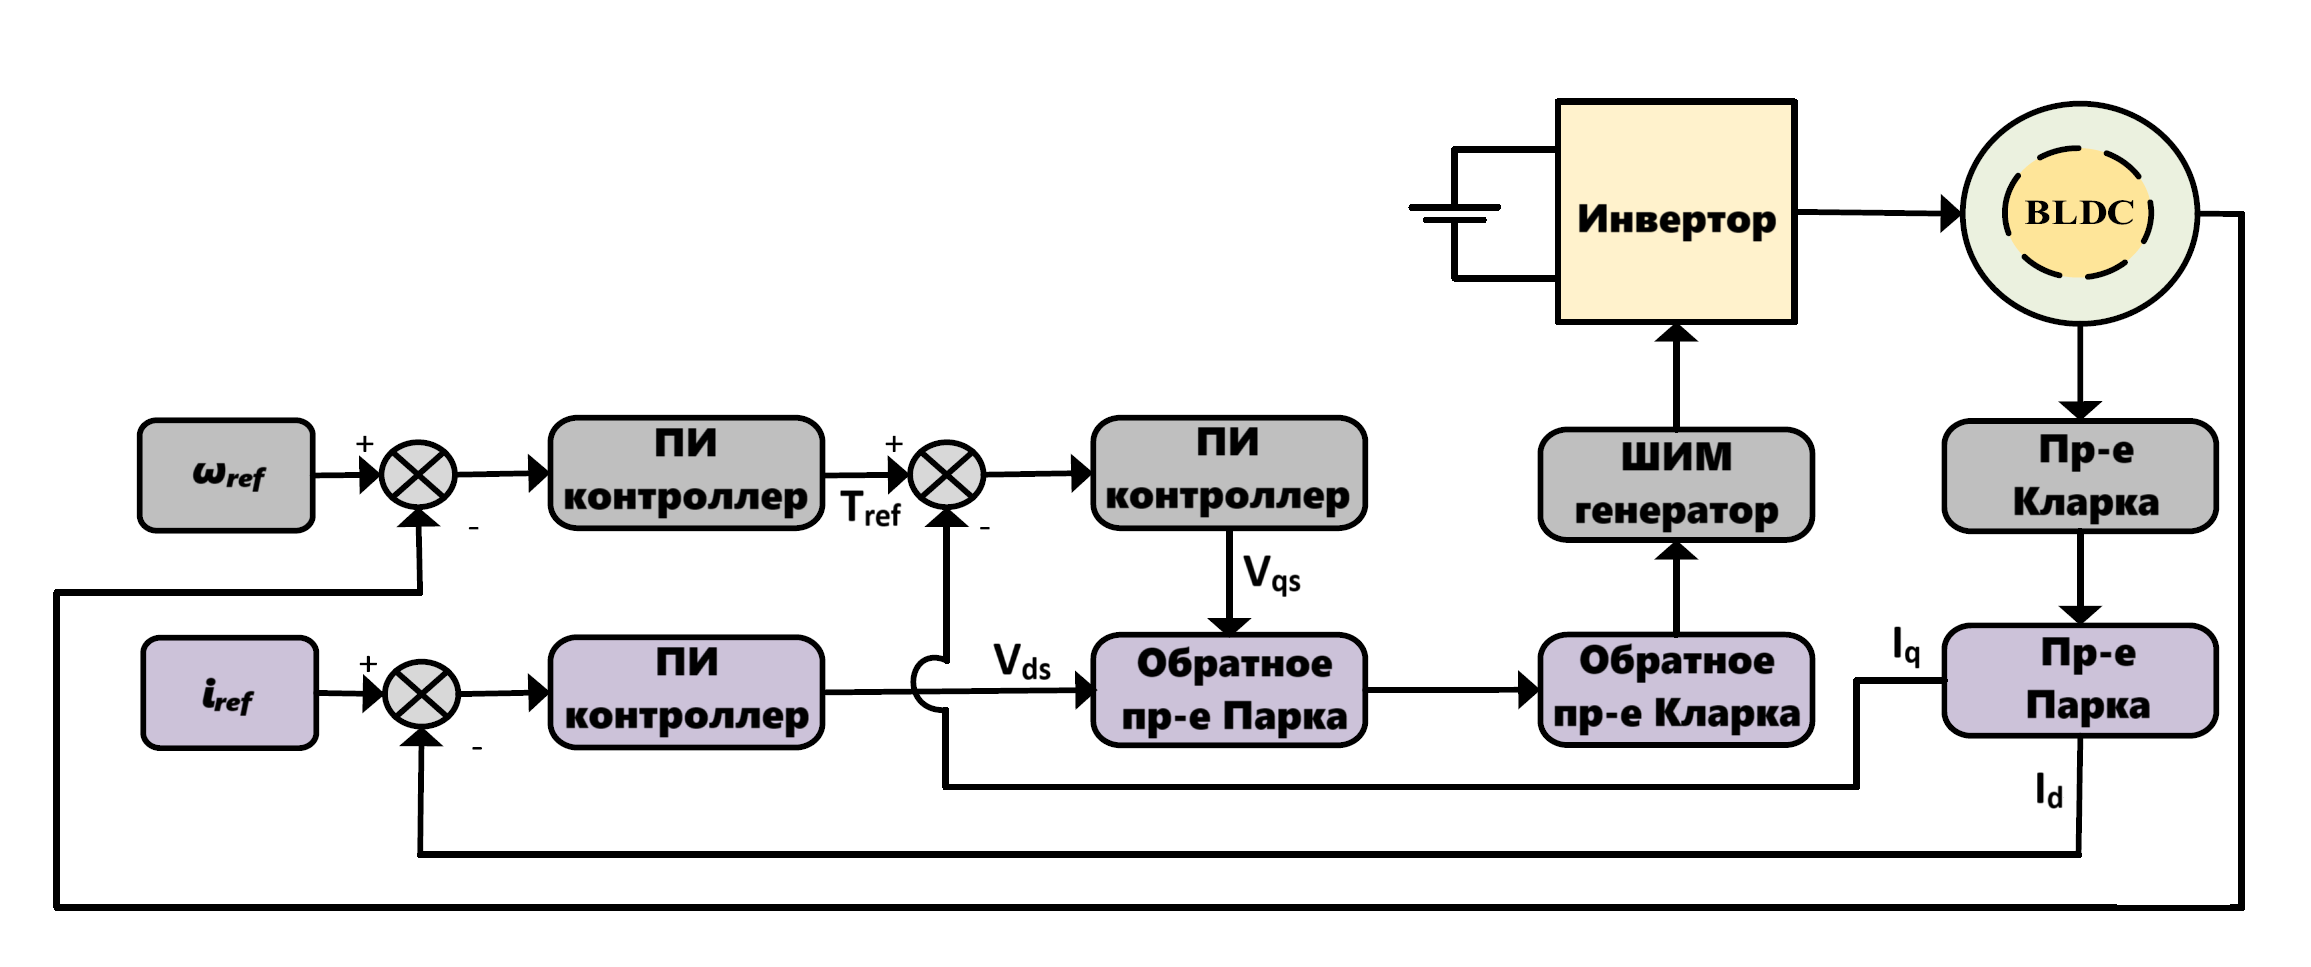
\includegraphics[width=\textwidth]{inc/img/foc.png}
\caption{Система регулирования для векторного управления \cite{art:bdlc_adv_control_techs}}
\label{pic:foc}
\end{figure}

Приведём алгоритм реализации данного типа управления \cite{art:foc_control}:
\begin{enumerate}
	\item Определение токов фаз двигателя с использованием соотношения:
	\[
		i_W+i_V+i_U=0
	\]
	\item Приведение трёх фазного тока к двухкоординатной системе с использованием преобразованиея Кларка:
	\begin{align*}
		&i_{\alpha}=i_W \\
		&i_{\beta}=(i_W+2i_V)/\sqrt{3}
	\end{align*}
	\item Двухкоординатная система преобразуется для согласования с потокосцеплением ротора (вращаем для совпадения с потоком ротора на основе его угла поворота $\theta$), т. е. выполняется преобразовние Парка (или преобразование во вращающуюся систему координат):
	\begin{align*}
		&I_d=i_{\alpha}\cos\theta+i_{\beta}\sin\theta\\
		&I_q=-i_{\alpha}\sin\theta+i_{\beta}\cos\theta
	\end{align*}
	\item Используем полученные векторы как входы двух ПИ регуляторов для формирования на выходе векторов напряжений --- $V_{dc}$ и $V_{qs}$. $I_d$ составляющая относится к току или потокосцеплению и в качестве референсного значения используется $0$ для уменьшения пульсаций момента. $I_q$ относится к моменту. 
	\item Используем обратное преобразование Парка:
	\begin{align*}
		&V_{\alpha}=V_{dc}\cos\theta-V_{qs}\sin\theta \\
		&V_{\beta}=V_{dc}\sin\theta+V_{qs}\cos\theta
	\end{align*}
	\item Используем обратное преобразование Кларка:
	\begin{align*}
		&V_W=V_{\beta}\\
		&V_V=(-V_{\beta}+\sqrt{3}V_{\alpha})/2\\
		&V_U=(-V_{\beta}-\sqrt{3}V_{\alpha})/2
	\end{align*}
	\item Полученные напряжения используем для генерации ШИМ сигнала на основе алгоритма SVPWM (пространственно-векторная широтно-импульсная модуляции) или SPWM (синусоидальная широтно-импульсная модуляция).
\end{enumerate}

Хоть данный метод и позволяет уменьшить пульсации момента, но для его нормального функционирования необходимо наличие датчиков положения ротора или очень точное его определение. Конечно, можно управлять и бездатчиковым методом, но обычно это выполняется с использованием наблюдателей положения и скорости на основе оценки противо-ЭДС, что требует больше вычислительных мощностей, больше информации о двигателе и является менее надёжным.

\section{Прямое управление моментом (DTC)}

В основе данного метода лежит оценка электромагнитного момента на основе тока и напряжения фаз статора и электрического положения ротора и его последующее регулирование. Возможная схема реализации этого алгоритма приведена на Рисунке \ref{pic:dtc}.

\begin{figure}[!h]
\centering
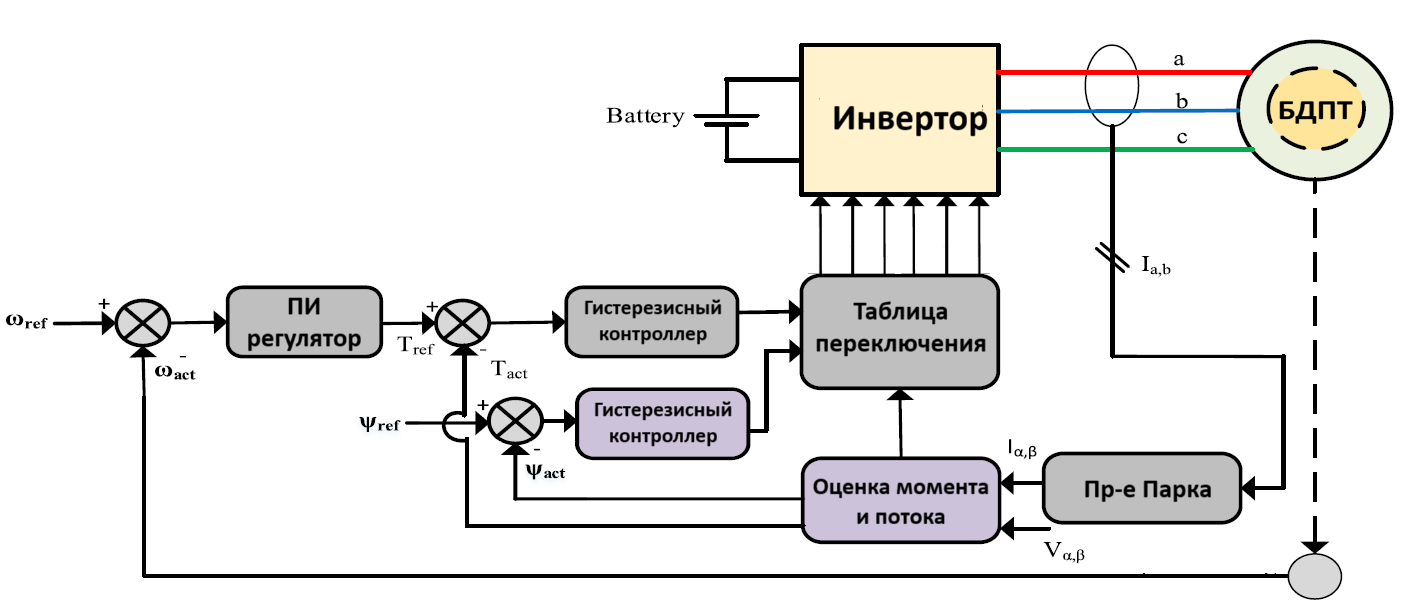
\includegraphics[width=\textwidth]{inc/img/dtc.png}
\caption{Система регулирования для прямого управления моментом \cite{art:bdlc_adv_control_techs}}
\label{pic:dtc}
\end{figure}

Алгоритм работы следующий:
\begin{enumerate}
	\item Выполнить переход к двумерной системе координат для тока и напряжения фаз путём преобразования Парка, определить угол положения ротора в электрических градусах
	\item Оценить на основе полученных данных электромагнитный момент двигателя и поток
	\item Получить ошибки по моменту и потоку, взяв за желаемое значение выход ПИ регулятора контура сокрости
	\item Пропустить ошибки через гистерезисные контроллеры, представляющие в самом простом случае функцию переключения с гистерезисом, которые на выходе имеют $1$ при превышении верхнего порога и $-1$ при выхода за нижний порог
	\item На основе полученных значений выходов и текущего положения ротора получить новые состояния ключей инвертора и либо замедлять ротор, либо ускорять для достижения нужного момента.
\end{enumerate}

Вместо гистерезисных контроллеров можно использовать ПИД регуляторы, но использование последних усложняет настройку регулятора и является более ресурсозатратным.

Этот метод является менее требовательным в плане вычислительных мощностей, обладает большей робастностью по отношению к параметрам двигателя и обладает лучшими динамическими свойствами по сравнению с векторным управлением. Однако для его нормального функционирования необходима большая частота работы регулятора, отчего зависят амплитуды пульсаций момента и скорости. Также он обладает меньшей эффективностью по сравнению с векторным управлением, но его простота позволяют просто реализовать и настроить (нужно найти подходящие парметры ПИ регулятора и выставить пороги гистерезисных регуляторов).